\documentclass{article}

% if you need to pass options to natbib, use, e.g.:
    \PassOptionsToPackage{square,numbers}{natbib}
% before loading neurips_2021

% ready for submission
% \usepackage{neurips_2021}

% to compile a preprint version, e.g., for submission to arXiv, add add the
% [preprint] option:
    \usepackage[preprint]{neurips_2021}

% to compile a camera-ready version, add the [final] option, e.g.:
    % \usepackage[final]{neurips_2021}

% to avoid loading the natbib package, add option nonatbib:
    % \usepackage[nonatbib]{neurips_2021}

\usepackage[utf8]{inputenc} % allow utf-8 input
\usepackage[T1]{fontenc}    % use 8-bit T1 fonts
\usepackage[colorlinks=true]{hyperref}       % hyperlinks
\usepackage{url}            % simple URL typesetting
\usepackage{booktabs}       % professional-quality tables
\usepackage{amsfonts}       % blackboard math symbols
\usepackage{nicefrac}       % compact symbols for 1/2, etc.
\usepackage{microtype}      % microtypography
\usepackage{xcolor}         % colors
\usepackage{graphicx}       % handling images
\usepackage{subcaption}     % subfigures and subcaptions
\usepackage{wrapfig}
\usepackage[export]{adjustbox}

\graphicspath{ {./img/} }
\bibliographystyle{abbrvnat}
\definecolor{Gray}{gray}{0.9}

\title{Going Against The Grain:\\India's Food Insecurity Problem}

\author{%
  Devank Tyagi \\
  Matrikelnummer 5966585\\
  devank.tyagi@student.uni-tuebingen.de\\
   \And
   Nitin Jain \\
   Matrikelnummer 5993679 \\
   nitin.jain@student.uni-tuebingen.de \\
}

\begin{document}

\maketitle

\begin{abstract}
  The paper paints a statistically-derived picture of India's role in the context of global food insecurity and the socio-economic conditions that are correlated with prevalent conditions. In particular, the factors of political instability and conflict, and income/employment disparities are discussed in detail as potential pain points.
  
  \textbf{GitHub repository:} \url{https://github.com/nitinjain96/food-security}
\end{abstract}

\section{Introduction: The Lion's Share}

The World Food Summit at Rome, 1996 \cite{rome1996} acknowledged the issue of hunger as a separate entity from malnourishment and decided to implement the World Food Summit Plan of Action, where the term 'food security' was formally defined. Hence, food security has been a well-defined concept since the beginning of this century and there has been a plethora of research on attempting to quantify this state of being unable to access adequate nutrition through any combination of physical, social or economic factors \cite{rome1996}. The most recent advancements in measuring the same are part of the Food and Agricultural Organization's (FAO) Voices of Hunger project \cite{cafiero}, which in turn gave rise to the Food Insecurity Experiences Scale (FIES) \cite{cafiero}. The FIES defines food insecurity to exist at different levels of severity (moderate, severe, undernourished) and provides a rationale and basis to measure each of them. They are defined as \cite{index_exp}:

- \textbf{Prevalence of Undernourishment (PoU):} \% of population whose daily food consumption habits are incapable of sustaining the energy levels needed to maintain functioning activity and health. This quantity is one of the longest-running and most prominent indicators for food insecurity.

- \textbf{Prevalence of Severe Food Insecurity in the Population (PSFI):} $\%$ of population which has been part of a household that has spent an entire day without consuming any nutrition while being affected by hunger, on multiple days, due to a lack of availability and/or physical/economic access.

- \textbf{Prevalence of Moderate or Severe Food Insecurity in the Population (PMSFI):} $\%$ of population living in households where at least one regular adult has had to reduce the quantity or quality of their regular diet, due to a lack of availability and/or physical/economic access.

A look at the numbers reveals the massive role that India plays in them. With an undernourishment count of 208.6 million people, one country alone accounts for about a third of this global issue (see Figure \ref{fig:1a}). To put the scale of the problem in perspective, a new country containing just India's undernourished population would be the world's 6th-most populous state. Clearly, a major proportion of the effort involved in solving world hunger must be directed towards the bottlenecks and chronic issues that bind India in this regard.

\begin{figure}

\begin{subfigure}{0.55\textwidth}
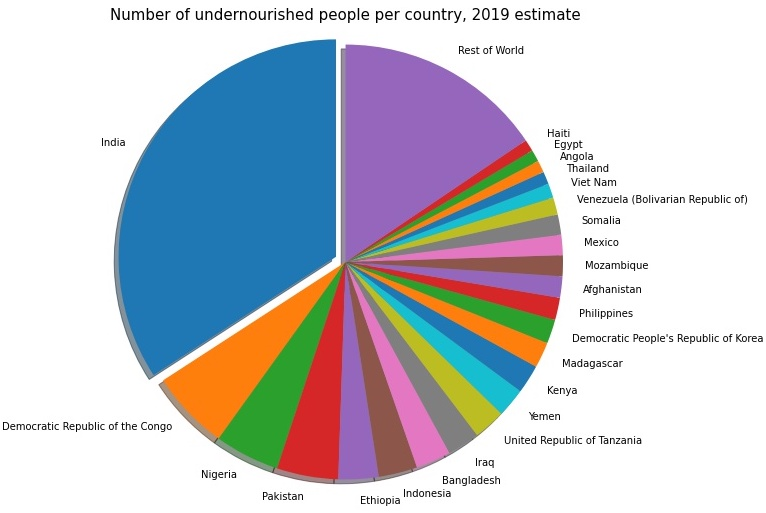
\includegraphics[width=\textwidth]{undernourished_breakup} 
\caption{India's undernourished population vs the rest}
\label{fig:1a}
\end{subfigure}
\begin{subfigure}{0.45\textwidth}
\vspace{9mm}
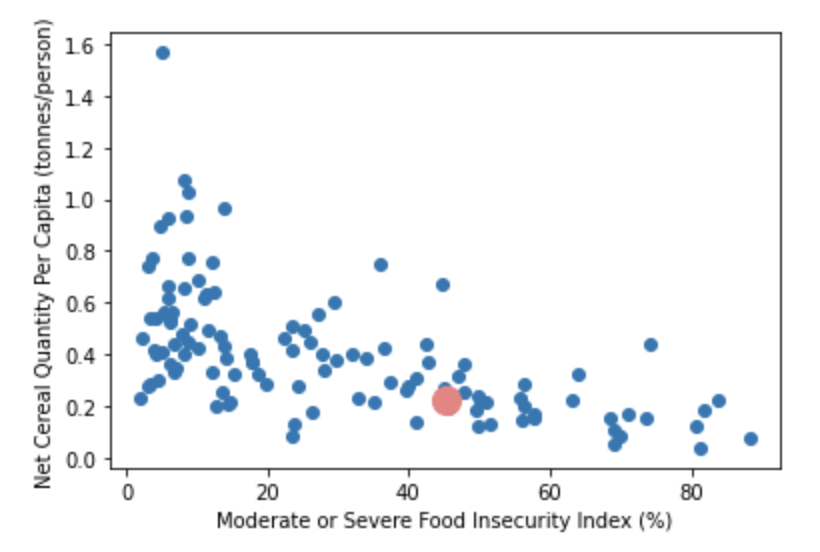
\includegraphics[width=\textwidth]{quant_vs_insecurity}
% \vspace{1mm}
\caption{Quantity per capita vs food insecurity}
\label{fig:1b}
\end{subfigure}

\caption{The Problem vs The 'Obvious' Cause}
\label{fig:figure1}
\end{figure}

\begin{figure}[b]
\begin{minipage}{.48\textwidth}
  \centering
  \vspace{5mm}
  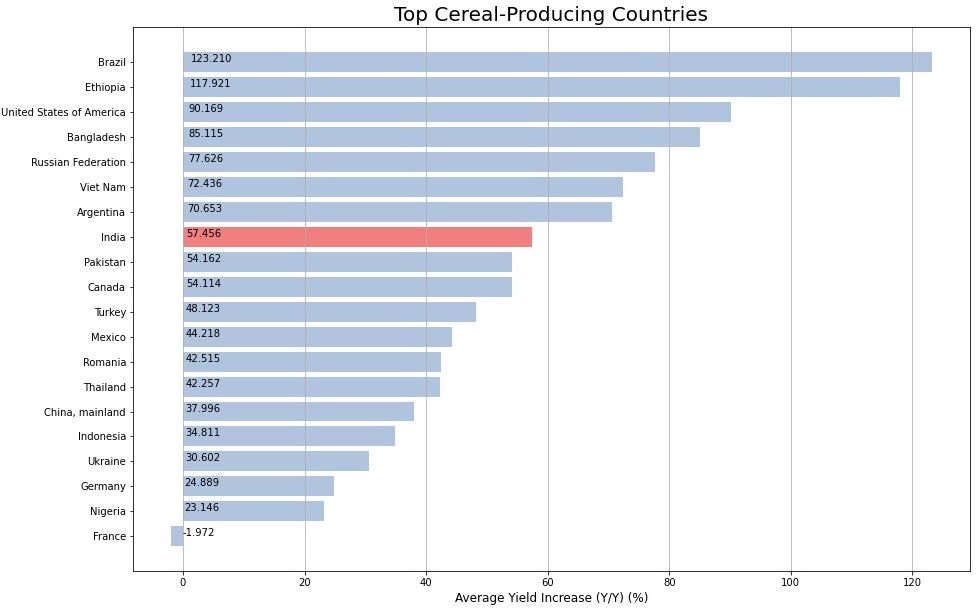
\includegraphics[width=\textwidth, left]{yield_increase}
  \captionof{figure}{Increase in India's average yield (Y/Y) compared to other top cereal-producing countries}
  \label{fig:2}
\end{minipage}%
\hfill
\begin{minipage}{.48\textwidth}
  \centering
  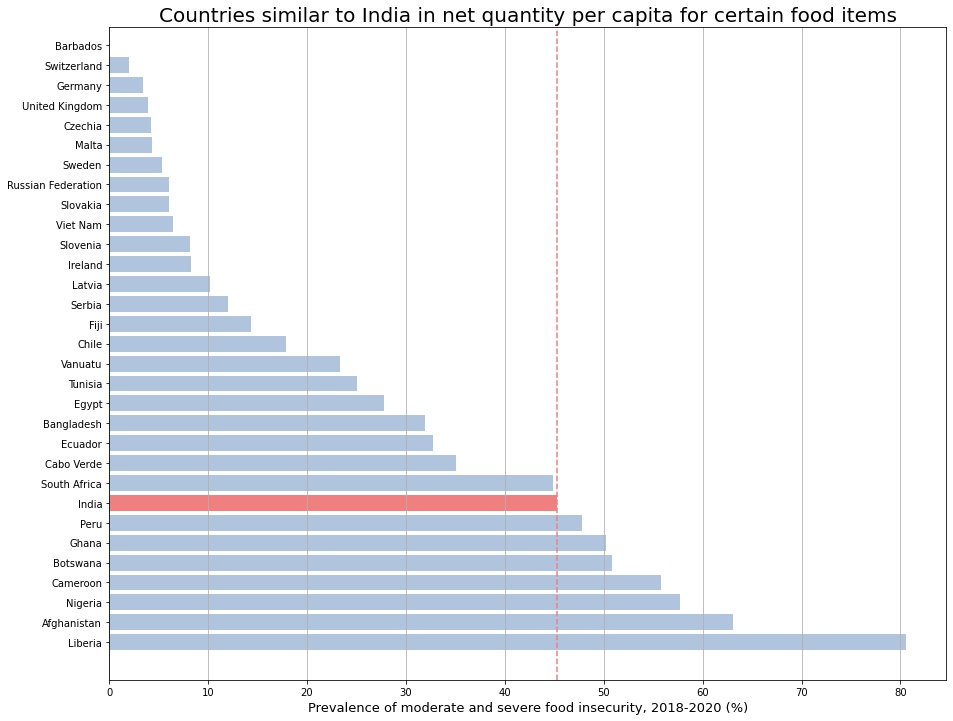
\includegraphics[width=\textwidth, right]{comparable_quantities}
  \captionof{figure}{A glimpse of the food insecurity index levels in countries with similar net quantities of varied foodstuffs per capita}
  \label{fig:3}
\end{minipage}
\end{figure}

\subsection{Sources of Data}

The data used for all statistical analyses and visualizations is publicly available, and primarily sourced from the \href{https://www.fao.org/faostat/en/#data}{FAOSTAT database}. All other sources will be cited as and when they are called upon.

\section{Analysis: An Interplay of Factors?}

\subsection{The 'Obvious' Cause}

The FAO defined the four pillars of food security \cite{pillars} as availability, access, utilization and stabilization. The first concern relates to the first pillar - whether the country possesses enough food to feed its masses. We collected data from the FAOSTAT database about the country's net quantity of foodstuffs, which was calculated simply as:

\begin{center}
    \emph{Net Quantity} = Production + Import - Export
\end{center}

Here, production refers to the domestic production of a food item while import and export are government policies on how much of that food item is sold or bought from other economies. In other words, a country that produces more food can be self-sufficient in its dietary requirements.

However, India does not face a challenge when it comes to domestic food production. In fact, it ranks among the top 5 producers in most important production indicators and is actually a net exporter of all major produced items, except pulses. Calculating the year-on-year increase in yield (production per unit area) also shows India to be in good stead (see Figure \ref{fig:2}), which indicates that the country's agro-technologies and methods have kept abreast with modern advancements (we consider cereals for most comparisons to stay attached to previous studies that measure production similarly). Hence, net quantity of food production cannot be taken in isolation to pinpoint food shortages, which is why we combine a population factor for normalization.

On normalizing the net quantities with the countries' total populations, a clearer picture begins to emerge. India's overcrowding problem \cite{overcrowding} sinks its lofty position among the top producers to reach 120 out of 186 countries for which data is available. Figure \ref{fig:1b} shows net quantity per capita to be negatively correlated with the aforementioned food insecurity indices, which intuitively makes sense. Should India simply stop exporting its produced goods and cater to its masses first?

In order to justify looking for other explanations, we looked for countries that had similar values for net quantity per capita and compared their PMSFI values against that of India's. Figure \ref{fig:3} shows that there are many countries which seem to be in similar situations without facing a substantial threat to their food security. The authors interpreted this as an indication to explore beyond the basic economic laws of demand and supply and investigate alternate existing correlations (if any).

\subsection{Linear Regression and Intrinsic Feature Selection}

The adopted approach for investigation involved selecting a curated set of features that could potentially play a role in influencing food insecurity across different geographies and timelines. This feature set included suggestions from existing literature alongside cross-discipline factors, such as country population, climatic changes, food commodity losses, government expenditure on agriculture, conflict and political instability, food inflation rates and gross domestic products adjusted for purchasing power parity (GDP-PPP). A consolidated dataset was created for this portion of the analysis (GDP-PPP data was sourced from the \href{https://data.worldbank.org/indicator/NY.GDP.PCAP.PP.CD}{World Bank data store}) and a regression model was fitted along the data while examining the data's linearity and ensuring low correlations between the selected features. The approach also involved imposing an intrinsic feature selection process through a regularization component. The model was fitted for both Lasso and Ridge regularization methods. We selected PoU as our food insecurity index due to the availability of a larger training set.

\begin{figure}[b]
\begin{minipage}{.48\textwidth}
  \centering
  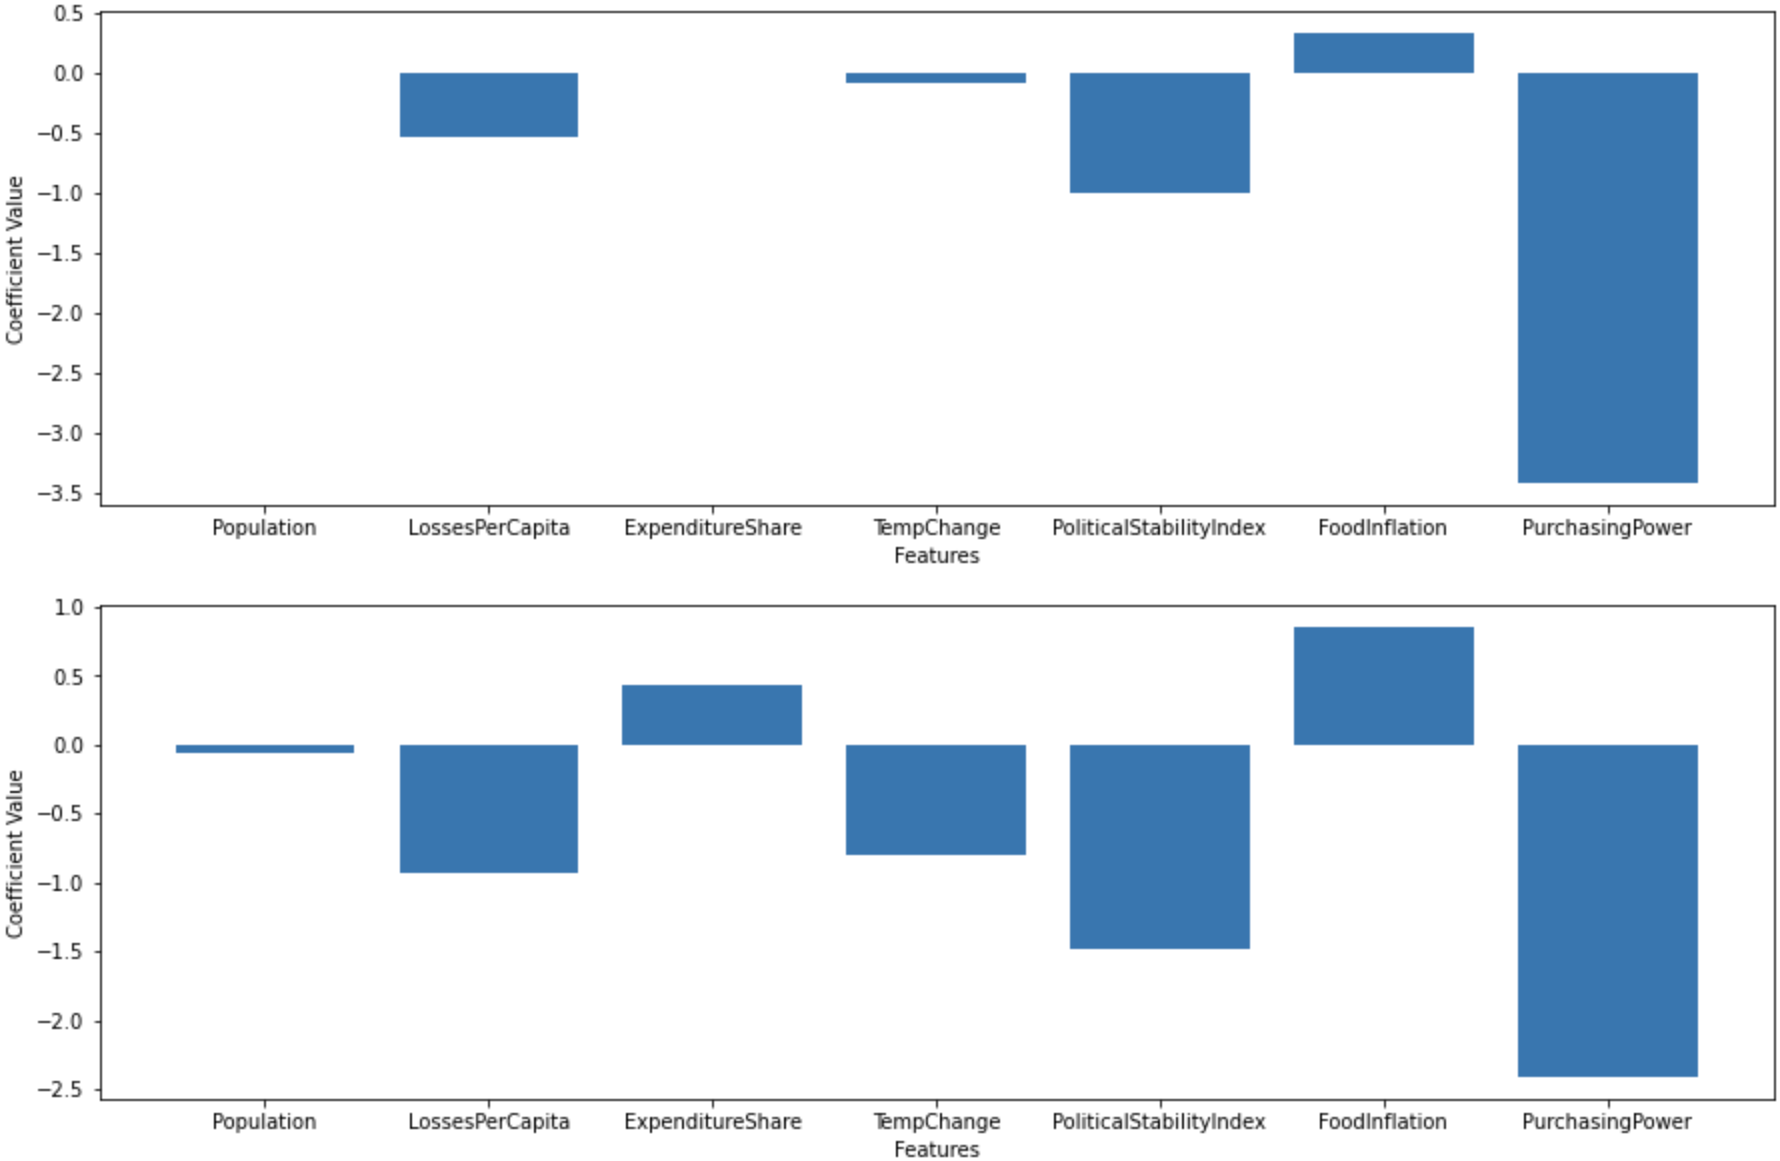
\includegraphics[width=\textwidth, left]{regression_results}
  \captionof{figure}{Finding important features related to PoU}
  \label{fig:4}
\end{minipage}%
\hfill
\begin{minipage}{.48\textwidth}
  \centering
  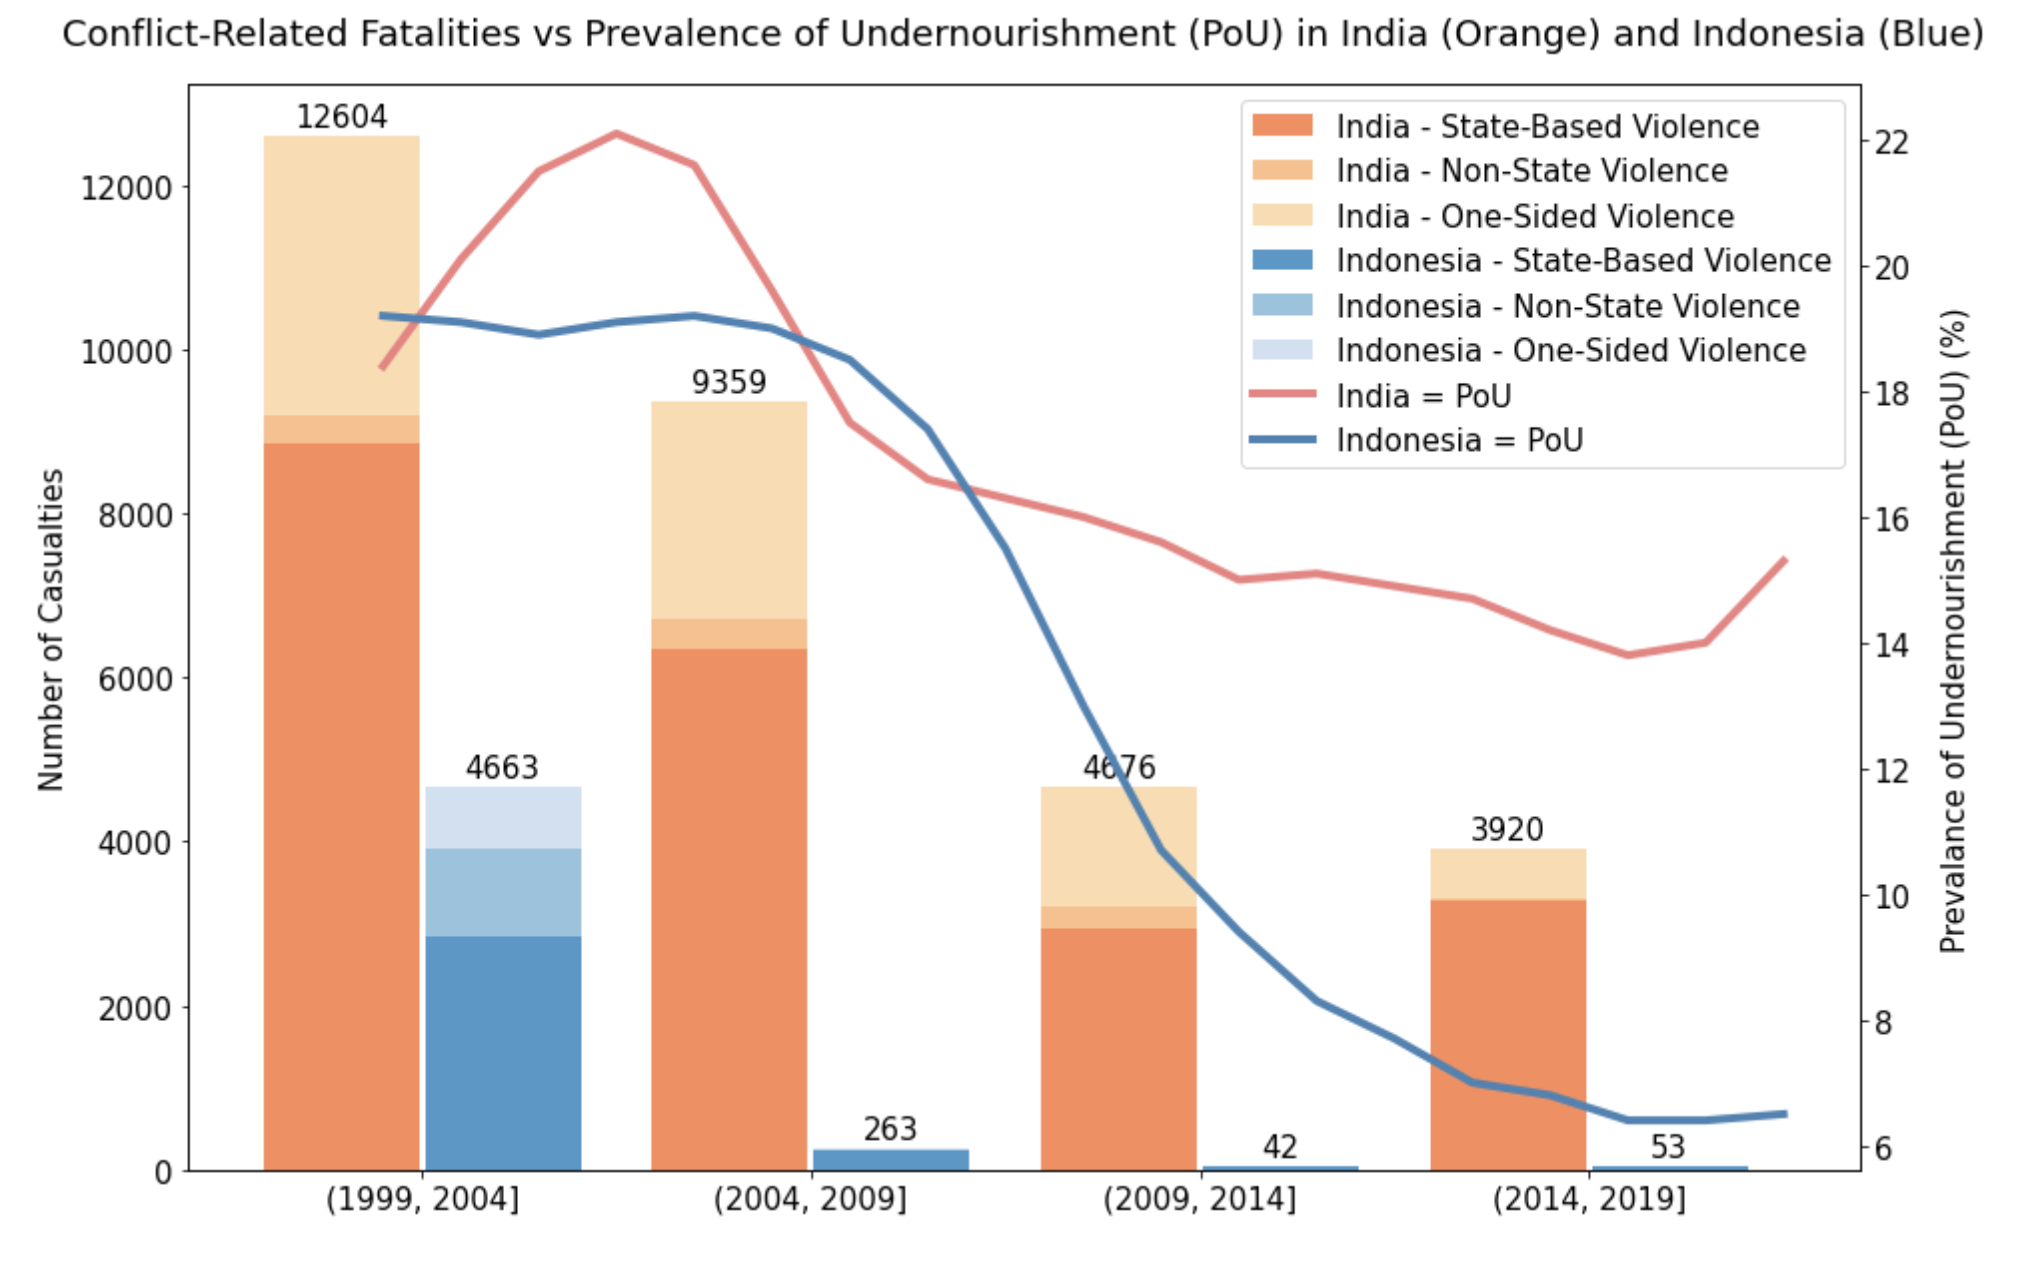
\includegraphics[width=\textwidth, right]{conflict}
  \captionof{figure}{Conflict/political instability and food insecurity}
  \label{fig:5}
\end{minipage}
\end{figure}

Figure \ref{fig:4} illustrates the results of training this model and retrieving important features through weight decay. The first notable result observed is the negation of 'Population' as a significant feature when predicting PoU, which assists in validating the results we obtained at the end of Section 2.1. The absence of importance to the share of government expenditure says that mere allocation of finances does not help either. The most significant features included conflict and political instability, GDP-PPP and food inflation rates. The following discussion takes a deeper look at the former two features, through the lens of a comparison with Indonesia, which was in a very similar food-insecure situation circa 2000 and has managed to show remarkable recovery in the next 20 years. Our selection of Indonesia was based on finding countries with similar PoU values and large population sample sizes.

\textbf{- Political Instability and Conflict:} Conflict-related data for the two countries was collated from the \href{https://ucdp.uu.se/encyclopedia}{Uppsala Conflict Data Program}, which tracks conflict-related information dating back to 1975. Figure \ref{fig:5} shows a timeline comparing the fatalities caused due to politically-charged violence and the incident PoU in those times. Indonesia's civil unrest in the early 2000s was directly related to a transition from autocracy to democracy, independent separatist movements and insurgencies. India continues to face challenges on most of these fronts, apart from external pressure from surrounding states and land disputes. This compromises their pursuit of the fourth pillar of food security and discourages focusing on internal hunger-related needs.

\begin{figure}

\begin{subfigure}{0.4\textwidth}
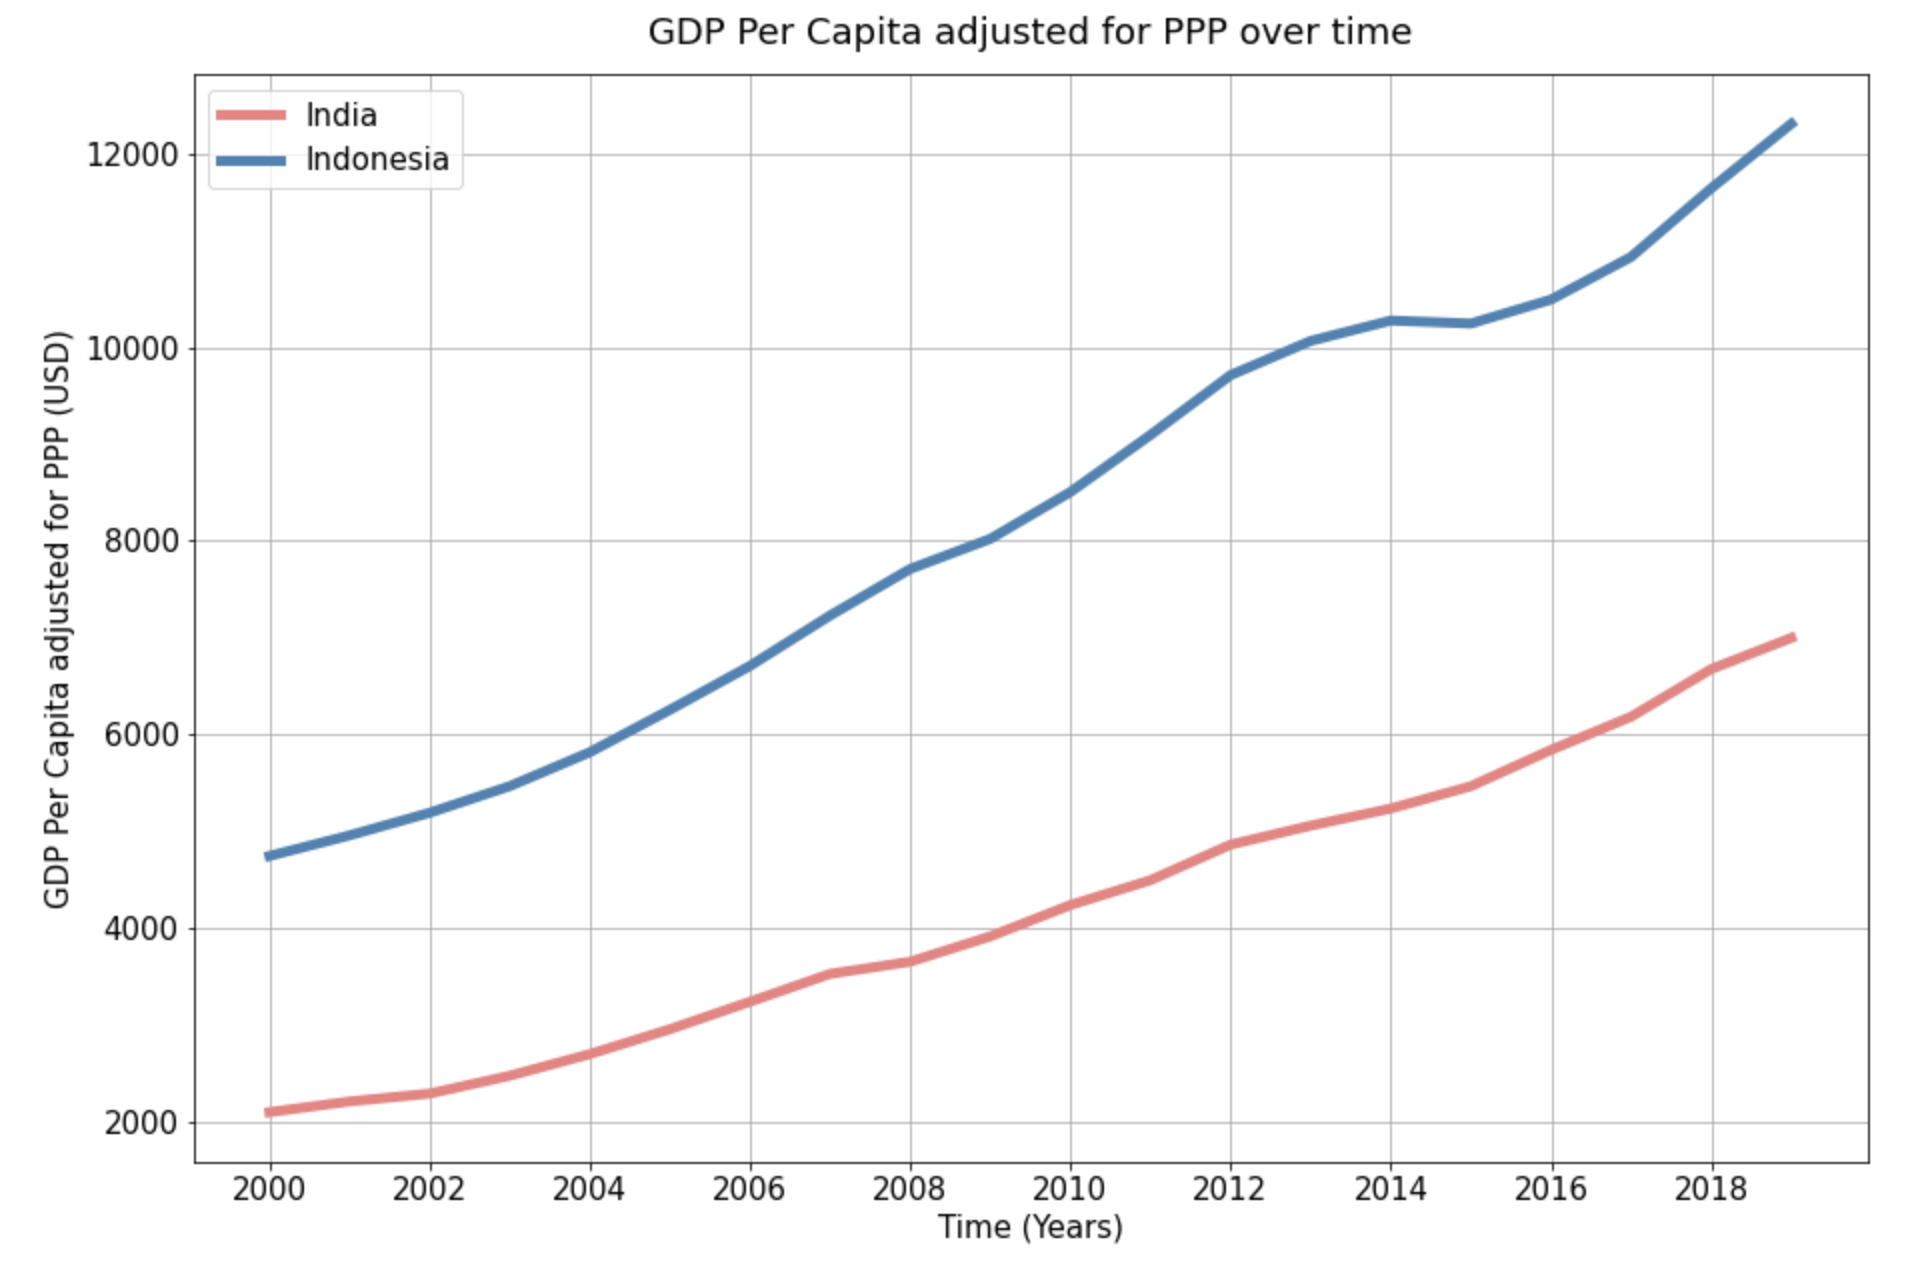
\includegraphics[width=\textwidth]{gdp_ppp} 
\caption{GDPs adjusted for purchasing power - following the same trend}
\label{fig:6a}
\end{subfigure}
\begin{subfigure}{0.6\textwidth}
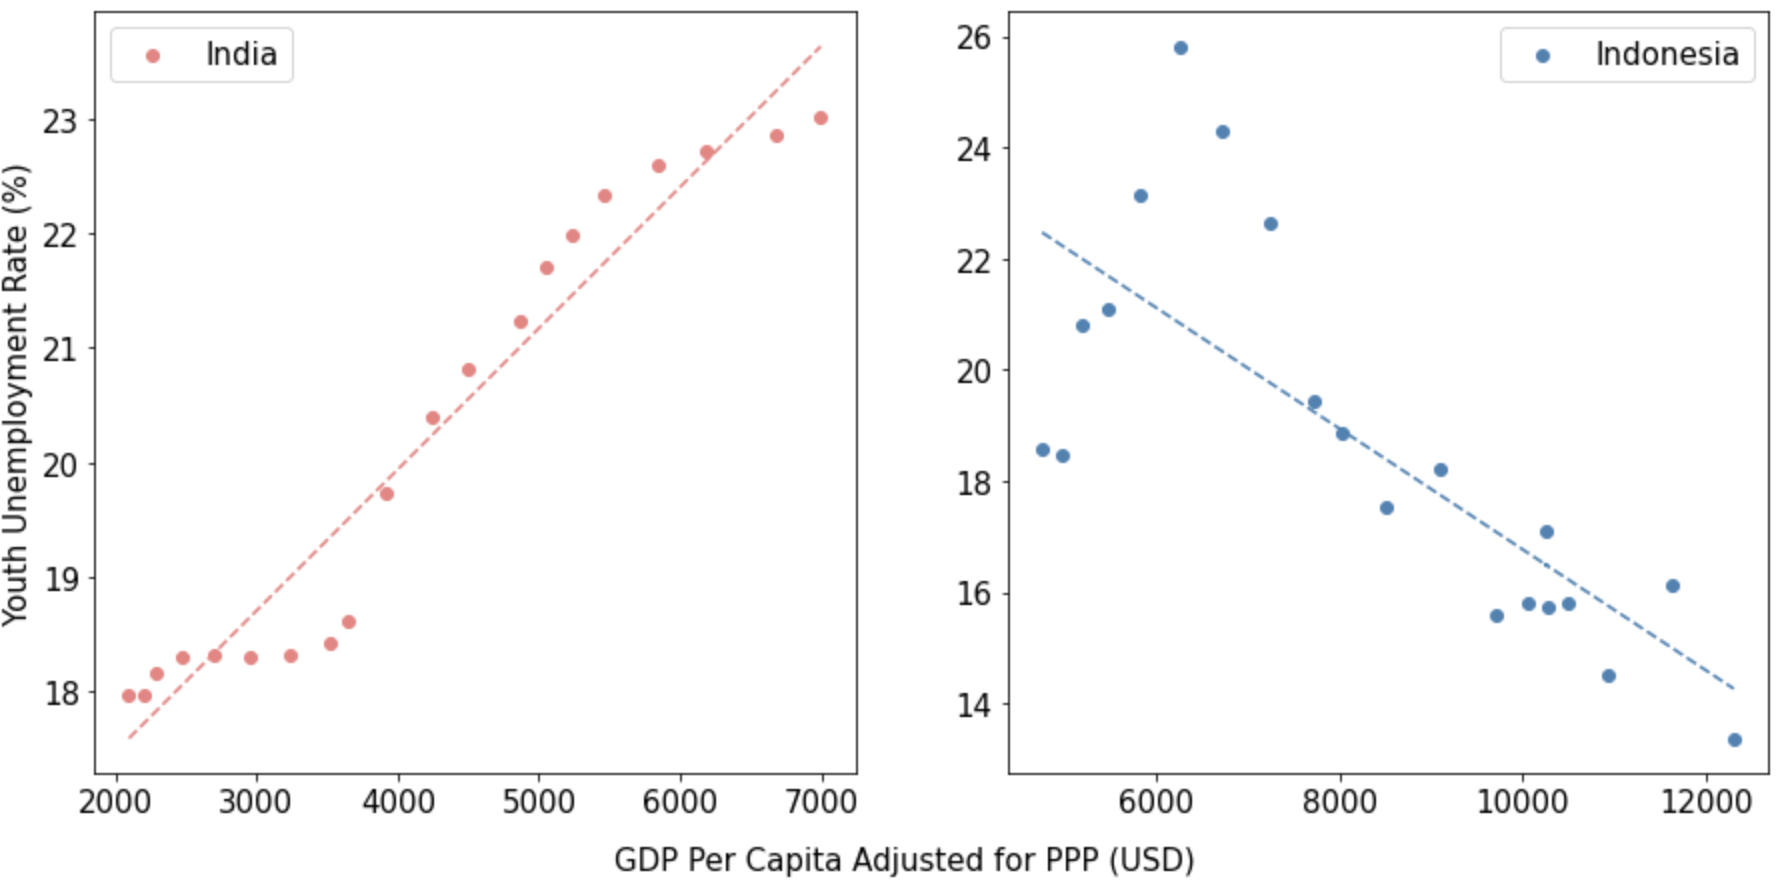
\includegraphics[width=\textwidth]{unemployment}
\caption{Breaking Okun's law: youth unemployment vs GDP-PPP}
\label{fig:6b}
\end{subfigure}

\caption{Economic comparisons: something's wrong.}
\label{fig:6}
\end{figure}

\textbf{- Gross Domestic Product per capita, PPP-adjusted:} At first glance, the corresponding statistics from both India and Indonesia do not show any stark differences, since the GDP-PPPs of both countries seem to be trending in similar directions. However, an interesting phenomenon is observed when these values are correlated with the corresponding \href{https://data.worldbank.org/indicator/SL.UEM.TOTL.ZS}{youth unemployment rates} over time. Contrary to the famous Okun's Law \cite{okunlaw}, India shows a corresponding increase in unemployment rates with rising GDP levels while Indonesia follows the expected trend. One possibility for this statistical anomaly is the rising income disparity between different economic and geographic sections \cite{india_disparity}, implying that positive growth of average income does not distribute evenly across the labour force and help alleviate the conditions of food-insecure households. This factor, coupled with a constantly-increasing food price inflation rate, may be putting a healthy diet beyond the reach of ever-expanding sections of the populace.

\section{Conclusion and Future Scope}

The prevalence of food insecurity in India depends on a multitude of intertwined factors that are not easy to isolate and even worse to try and mend. Nevertheless, it remains an important exercise to analyze and break the problem down into simpler subsections that can be isolated and targeted in particular - an exercise that proved very beneficial in Brazil \cite{brazil}, using the same indicators of insecurity. Future extensions with larger limits would allow an in-depth perusal of the other factors with a potential plan of action, preferably at an individual citizen's level.

{
\small
\bibliography{sample}
}

\end{document}